\chapter{Analysis}

In this chapter, we will be doing problem analysis. We will dive deeper into the problem we are addressing, and why we believe it to be a problem in the first place. We also compare source code with our definition of pseudocode, to get a better feel for their differences. Lastly, we will discuss some of the existing approaches, that already solve parts of the problem.

\section{Problem Definition}

Let us outline the problem at hand more concretely. Simply put, we aim to present computer programs at different abstraction levels, whilst maintaining their underlying ideas. The concept is nothing new, but has traditionally been carried out manually by the programmer. We believe there is a benefit in centralising resources and automating the conversion part. \\

There are several use cases where it is useful to display source code in a different light. Mainly in computer science education, where the goal often is to teach students concepts in a programming language agonstic way. It could also be used by researchers to exchange ideas across preferred programming languages. \\

When teaching computed programming at e.g. university level, it is important to distinguish between a student's grasp of computer science topics and their mastering of a particular programming language. Even though a student struggles with the syntax of, say, Go, it does not mean they have an inability to understand the broader concepts. Thus, the teacher can level the playing field by opting for pseudocode when introducing new concepts. \\

Shackelford and LeBlanc Jr. go as far as to say that using pseudocode can ``free students from the myriad of programming language details that annoy and distract attention from the core issue of algorithmic problem solving''~\cite{dislikeProgLang}. This could also apply to researchers who might wish to exchange ideas across different programming languages. \\

On the other hand, flowcharts can offer a visual approach to understanding programming concepts. If a teacher presents their ideas in the form of flowcharts, the classroom can focus on understanding its underlying ideas. If the ideas are presented in source code, students might be distracted by syntactic nuances of the teacher's preferred programming language. \\

In the context of our problem, and the remainder of this thesis, we treat both traditional pseudocode and flowcharts as pseudocode. To make a distinction, we introduce the terms \textbf{Text based pseudocode} (TBP) and \textbf{Image based pseudocode} (IBP).

\section{Comparing Source Code with Pseudocode}

In this section we aim to show how the same computer program can be presented in three different levels of abstraction. The first one will be source code written in a popular programming language, while the latter two will be TBP and IBP. \\

The program in question is a solution to the \texttt{FizzBuzz problem}, commonly presented in entry level interview settings and beginner programming exercises. The input is an integer \texttt{n}, and the output depends on the integer's value: if \texttt{n} is divisible by 3 and 5 we return \texttt{FizzBuzz}, if \texttt{n} is divisible by 3 but not 5 we return \texttt{Fizz}, and if \texttt{n} is divisible by 5 but not 3 we return \texttt{Buzz}. If \texttt{n} is not dividible by either, we simply return \texttt{n}. \\

\Cref{FizzBuzzGo} shows the program written in the Go programming language. \Cref{FizzBuzz with Algorithm2e.} and \Cref{FizzBuzzTikZ.} show the same program, but with TBP and IBP, respectively. \\

The biggest difference between the Go program and the pseudocodes, is that the former contains boilerplate code. For instance, we have to declare which package the file belongs to. In our case, we simply call the package \texttt{fizzbuzz}. We also have to import a package for converting integers to strings, to convert \texttt{n} before returning it in the last case. This is because functions can only have one return type in Go. \\

\begin{lstlisting}[caption={A Go program solving the FizzBuzz problem.}, captionpos=b, label={FizzBuzzGo}]
package fizzbuzz

import "strconv"

func FizzBuzz(n int) string {
    if n%3 == 0 && n%5 == 0 {
        return "FizzBuzz"
    } else if n%3 == 0 {
        return "Fizz"
    } else if n%5 == 0 {
        return "Fizz"
    }
    return strconv.Itoa(n)
}
\end{lstlisting}

The main similarity between the source code and the TBP is that both versions resemble an executable program. People familiar with programming will likely understand the logic conveyed by the pseudocode, even if they have no prior experience with the Algorithm2e library. Both versions present each instruction as sequential lines, and employ common program language syntax like \texttt{else if} and \texttt{return}. \\

One of the differences is how the TBP version has a specific place for describing input and output. With Go, we would either have to them with comments, or leave the users to guess the desired output. \\

Additionally, since TBP is intentionally not executable, we given total control over what we wish to include and exclude. We are free to emphasise particular parts, and also omit non-essential details. This allows us to increase the understanding of our programs more easily. \\

\begin{figure}[ht]
    \centering
    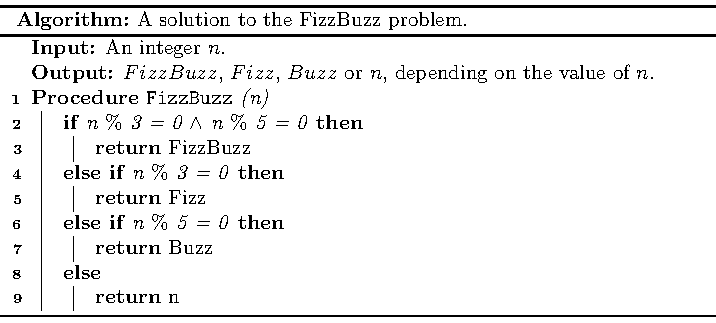
\includegraphics[scale=.95]{assets/chapter3/FizzBuzzAlgorithm2e.pdf}
    \caption{Pseudocode of a program solving the FizzBuzz problem.}
    \label{FizzBuzz with Algorithm2e.}
\end{figure}

All the same can be said for the IBP version, that does not particularly resemble the original source program. In appearance, they are on very different abstraction levels. Whereas the code is written in sequential lines, the flowchart shows colourful shapes wandering off in different directions. \\

The spacing and colourfulness of IBP can make it easier to isolate parts of the program, and to see more precisely how each part works individually. It also makes it easier to follow each path of the program, compared to the Go program, where the order of function calls and scoping of if-statements can confuse even more seasoned programmers. \\

The notation stays much the same, but since flowcharts are not executable, we can again opt for more precise mathematical notation to describe expressions, and exclude static properties like types.

\begin{figure}[ht]
    \centering
    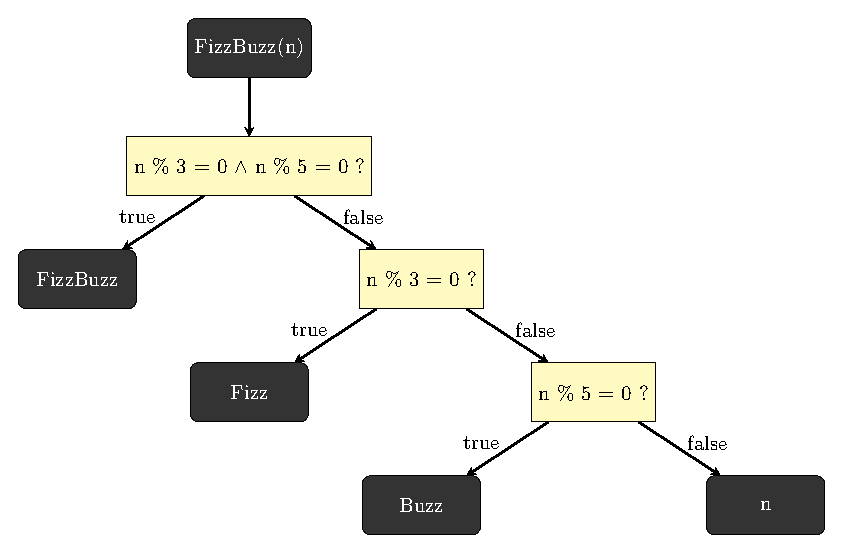
\includegraphics[scale=.75]{assets/chapter3/FizzBuzzTikZ.pdf}
    \caption{Flowchart of a program solving the FizzBuzz problem.}
    \label{FizzBuzzTikZ.}
\end{figure}

\section{Previous work}

This section covers selected works and software that have already solved parts of the problem, in their own right. The first section shows different approaches to convert source code to pseudocode, by applying machine learning. \\

The second section shows interplay between source code and flowcharts, converting one to the other. We also discuss the most basic way of converting between these formats: by doing it manually.

\subsection{Pseudocode}

Despite TBP being used in so many textbooks, online courses and published papers, there are not an overwhelming amount of source code-to-pseudocode editors currently available online. Majority of research on this topic, to the best of our knowledge, seems to be centered around machine learning approaches.

\subsubsection{Manual Approach}

The benefits of manually pseudocode manually, is that we are void of any restrictions. We can select the desired abstraction level, we can emphasise what we wish, and the visual formatting is entirely up to us. \\

The biggest downside is the extra effort it requires to maintain two versions of our computer programs. We might change our source code but forget to update the pseudocode. Sometimes we might fail to consistently rename variables, or accidentally misplace parentheses and demonstrate a wrong formula.

\subsubsection{Machine Learning Approach}

In 2015, Oda et al. introduced \textbf{Pseudogen}, a tool for converting Python source code to pseudocode using a statistical machine translation (SMT) approach~\cite{pseudogen}. The pseudocode produced is really a line-for-line description of the Python program provided as input. \\

SMT is a technique to train machine learning models on samples of translations supplied by humans~\cite{whatIsSMT}. It is most commonly used for translating between two natural languages, for instance from English to Italian. In the context of Pseudogen, SMT is used to translate Python to English and Japanese. \\

Despite being a programming language notoriously known for sticking to natural language where many others use more technical notation,\footnote{The best example might be \textbf{\texttt{and}} over \textbf{\texttt{\&\&}}, and \textbf{\texttt{or}} over \textbf{\texttt{||}}, that we find in more or less all other programming languages.} Python still bears the mark of being a programming language. People unfamiliar with programming might still struggle to understand some of the more technical aspects of its syntax, like decorators and closures. \\

\Cref{pseudogenExample1} shows an excerpt taken from the 2015 paper where Pseudogen was first presented. It displays Python source code on the left, and pseudocode on the right. The program in question is an algorithm that solves the \texttt{FizzBuzz} problem, that we also looked at in Section 3.2. \\

\begin{figure}[ht]
    \centering
    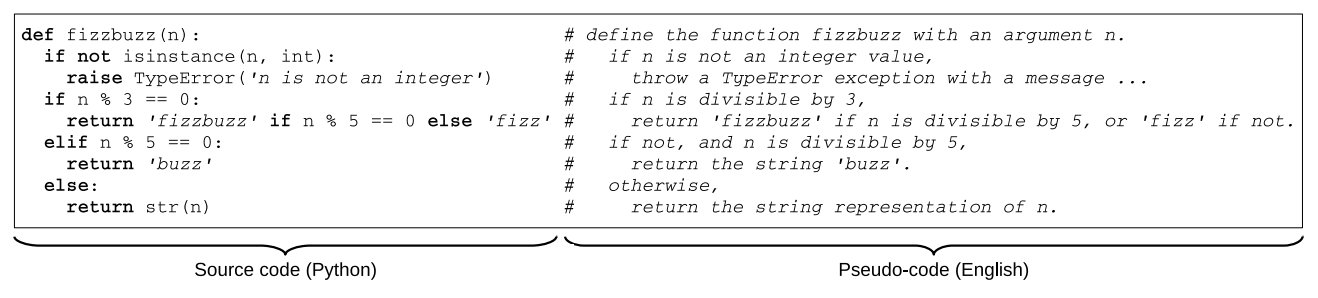
\includegraphics[scale=0.52]{assets/chapter3/odaetal.png}
    \caption{Python source code translated to pseudocode with Pseudogen. This example is not generated by us, but taken directly from~\cite{pseudogen}.}
    \label{pseudogenExample1}
\end{figure}

Since Pseudogen will translate each line in a servile manner, all error handling is translated too. \Cref{Error handling in Python.} shows some error handling in Python, and \Cref{Error handling in Pseudogen.} shows the result from transpiling it with Pseudogen. The result is considerably more verbose, which defeats some of the point with Python, whose syntax tends to be elegant and succinct, already closely resembling English. \\

\begin{lstlisting}[caption={Error handling in Python.}, captionpos=b, label={Error handling in Python.}]
except ValueError as e:
    print(e)
\end{lstlisting}

\begin{lstlisting}[caption={Pseudocode version of \Cref{Error handling in Python.} generated with Pseudogen. This example is not generated by us, but copied from a video on their website.}, captionpos=b, label={Error handling in Pseudogen.}]
# If ValueError, renamed to e, exception is caught.
    # Call the function print with an argument e.
\end{lstlisting}

Another example is visible in \Cref{listComprehensionPython} and \Cref{listComprehensionPseudogen}, where list comprehension has been translated quite literally. It is plausible to assume people with backgrounds in academia might favour the Python version to the transpiled one, as it closely resembles how we would write set comprehension in mathematics~\cite[11]{setComprehension}. \\

\begin{lstlisting}[caption={A list comprehension of applying f(n) to integers in the range -10 to 10, and placing the results in a list.}, captionpos=b, label={listComprehensionPython}]
a = [f(n) for n in range(-10, 10)]
\end{lstlisting}

\begin{lstlisting}[caption={Pseudocode version of \Cref{listComprehensionPython} generated with Pseudogen. This example is not generated by us, but copied from a video on their website.}, captionpos=b, label={listComprehensionPseudogen}]
# Call the function f with an argument n for every
  n in range of integers from range 10 negative
  integer 10, substitute the result for a
\end{lstlisting}

In 2018, Alhefdhi et al. introduced \textbf{Code2Pseudocode}, a machine learning model that also utilises machine translation techniques. The output follows the format of Pseudogen, but rather than sticking with SMT, they have opted for Neural Machine Translation (NMT). \\

NMT is another variant of machine translation, inspired by neural networks in the human brain. The approach has become the standard for large-scale machine translation, according to a 2019 review and survey carried out by Stahlberg~\cite{nmtOverSmt}. \\

\begin{figure}[ht]
    \centering
    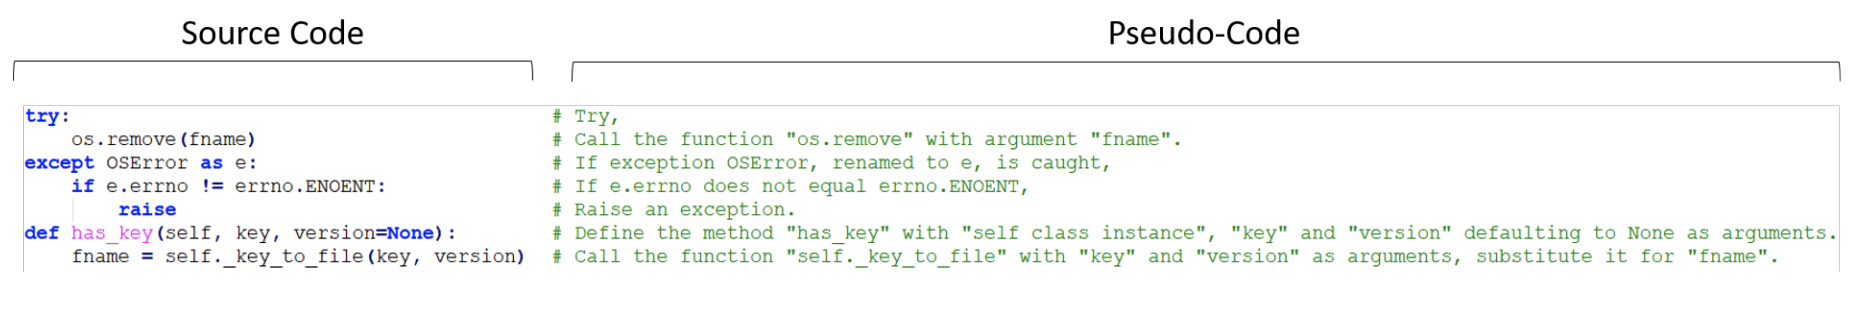
\includegraphics[scale=.37]{assets/chapter3/Code2Pseudocode.png}
    \caption{Python source code translated to pseudocode with Code2Pseudo -code. This example is not generated by us, but taken directly from~\cite{code2pseudocode}.}
    \label{code2Pseudocode}
\end{figure}

\Cref{code2Pseudocode} shows an excerpt taken from the 2018 paper where Code2Pseudocode is presented. It is similar to \Cref{pseudogenExample1} in nature: Python source code on the left, and generated psudocode on the right. The program tries to remove a file from the computer, and raises an error if it fails. \\

Since neither Pseudogen nor Code2Pseudocode have knowledge of Python itself, the descriptions they provide are very general. For instance, the pseudocode in \Cref{pseudogenExample1} does not explain what an ``exception'' is, or what it really means to ``throw an exception''. Likewise, the pseudocode in \Cref{code2Pseudocode} does not tell us that \texttt{os.remove(fname)} will actually remove \texttt{fname} from our computer, only that it calls \texttt{os.remove()} with \texttt{fname} as argument. \\

Truthfully, recent advancements in artificial intelligence are able to do much of this for us now. For instance, the freely available prompt-based tool ChatGPT is now able to do this job entirely on its own.\footnote{It is currently available here: \url{https://chat.openai.com/}.} Additionally, rather than giving a line-for-line translation, it is able to give a concise summary of what the program actually does. \Cref{gptfizz} and \Cref{gptos} are examples of asking it to summarise the Python programs we saw in \Cref{pseudogenExample1} and \Cref{code2Pseudocode}, respectively. \\

\begin{figure}[ht]
    \centering
    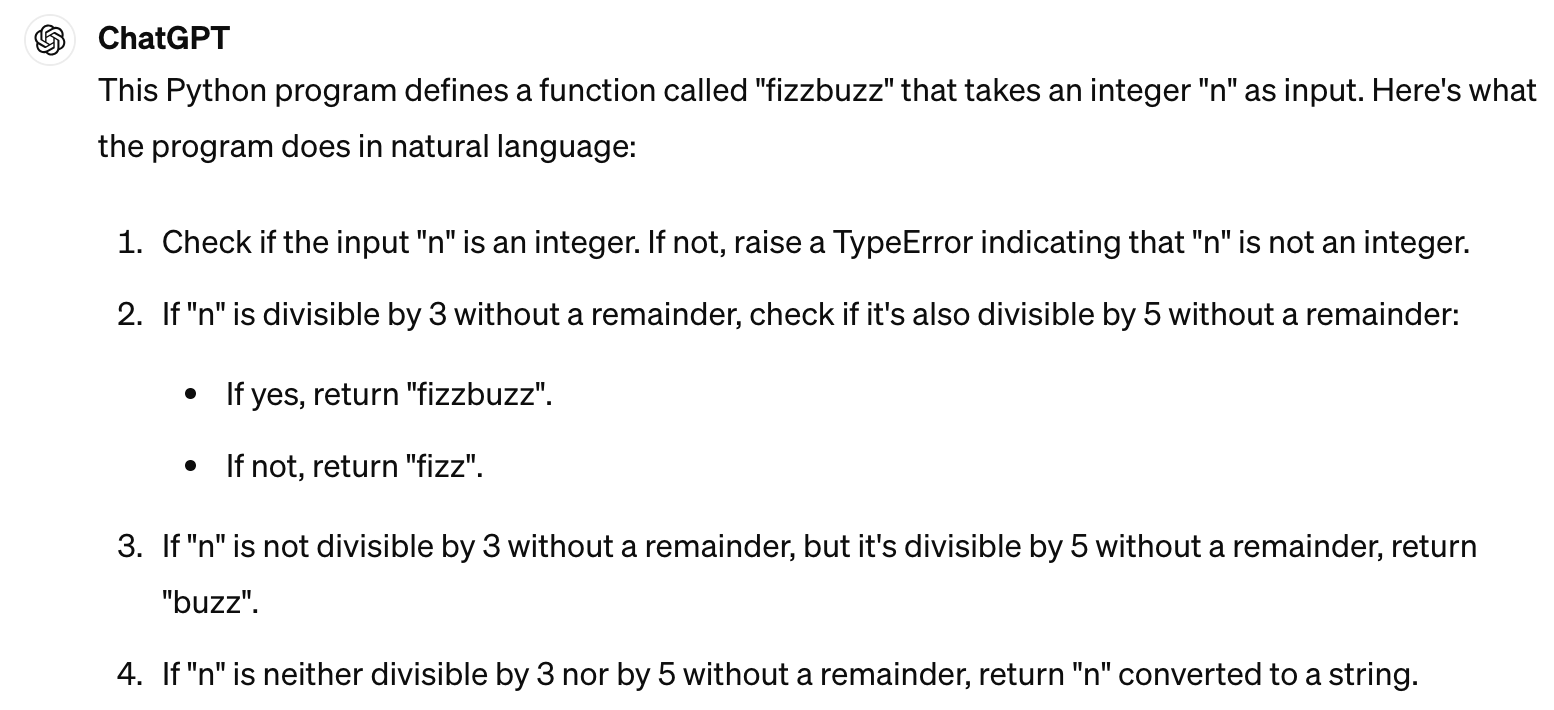
\includegraphics[scale=.45]{assets/chapter3/gptFizzbuzz.png}
    \caption{ChatGPT giving a summary of the Python code from \Cref{pseudogenExample1}.}
    \label{gptfizz}
\end{figure}

\begin{figure}[ht]
    \centering
    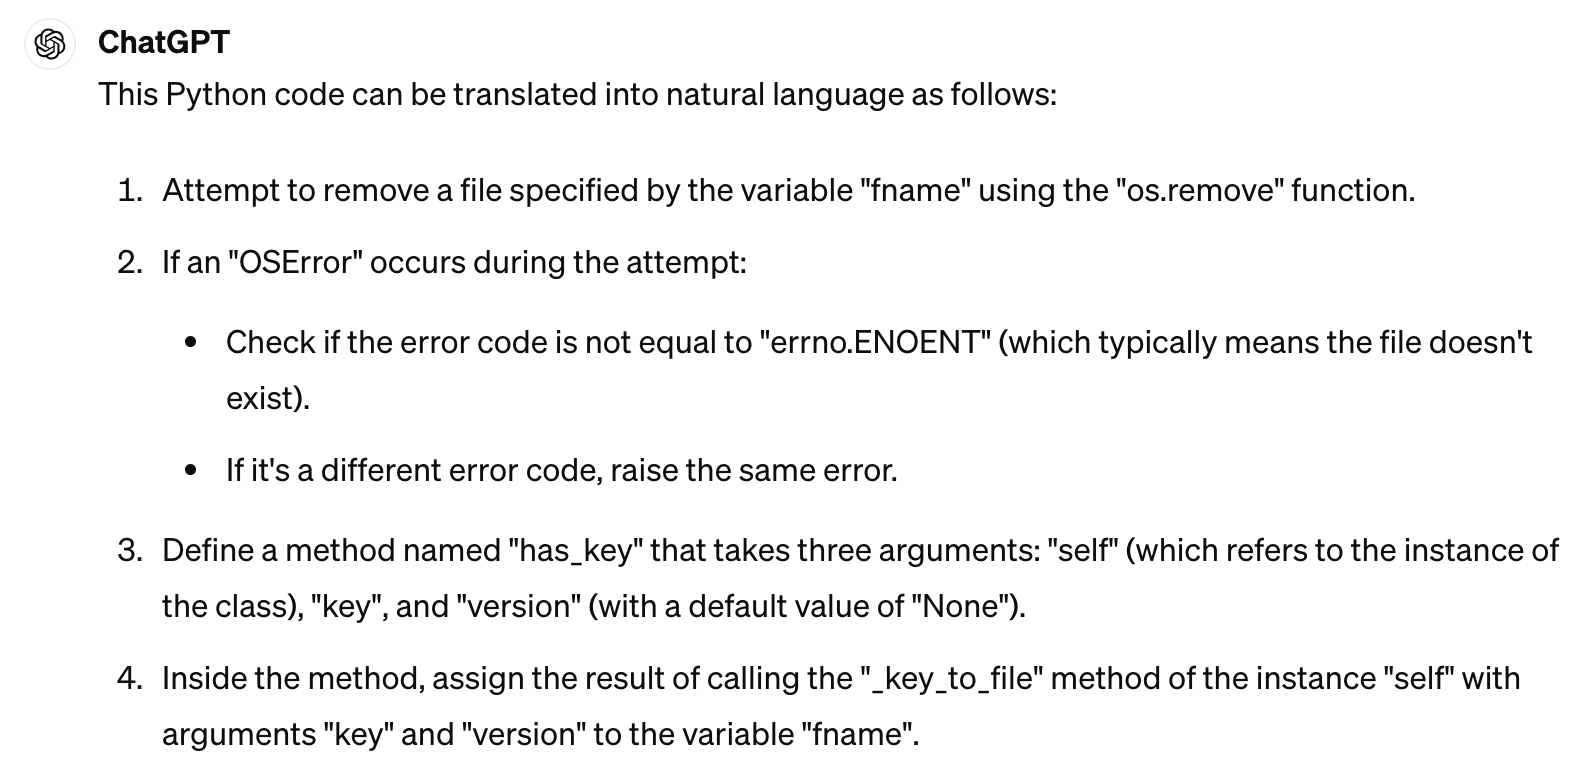
\includegraphics[scale=.45]{assets/chapter3/gptOS.png}
    \caption{ChatGPT giving a summary of the Python code from \Cref{code2Pseudocode}.}
    \label{gptos}
\end{figure}

\subsection{Flowcharts}

There is a good deal of research advocating for using flowcharts as an alternative to traditional code when demonstrating computer science concepts~\cite{flowchartsAreGood1, flowchartsAreGood2, flowchartsAreGood3}. Research on ways to construct corresponding flowcharts from source code, however, is not plentiful. In this section, we will look at a 2015 paper, as well as online editors providing our desired transpilation. \\

\subsubsection{Manual Approach}

Like with TBP, the main benefit of translating our source code to flowchart manually is the lack of restrictions. We are free to use our preferred drawing tool, and can choose to emphasise parts of our program just the way we like - with colours, shapes, arrows, and more. \\

However, if we were to change the main ideas of our code, we would have to draw the flowchart again from scratch. This means that the time spent on making the original IBP version is - to a certain extent - wasted. \\

Another burden is that we are entirely responsible for how the corresponding flowchart should look. By doing this process manually, we have to spend time on the design, which is actually unrelated to the actual program logic.

\subsubsection{Research-driven Approach}

In 2015, Kosower et al. introduced \textbf{Flowgen}, a flowchart-based documentation framework for C++. The tool converts annotated C++ programs to high-level UML activity diagrams, providing a description of the code's dynamic behaviour~\cite{flowgen}. \\

Flowgen extracts control flow parts of a program, as well as annotations initiated by \texttt{//\$}, to build flowcharts for each function or method. Understanding what C++ programs do is outside the scope of this thesis, with the relevant part being how Flogen represents a program written in executable source code as a flowchart. \\

\Cref{c++prog} shows a C++ program with Flowgen annotations, and \Cref{flowgenExample} shows the corresponding flowchart created by Flogen. We have not generated this flowchart ourselves, instead it is taken directly from~\cite{flowgen}. \\

\begin{lstlisting}[caption={A C++ program.}, captionpos=b, label={c++prog}]
#include \\aux.h''
#include <iostream>
int main()
{
    int control flag=0;
    //$\textdollar$ ask user whether to proceed
    std::cin >> control flag;
    if (control flag==1){
        //$\textdollar$ call shower
        // pointer to the object VINCIA
        VINCIA* vinciaOBJ = new VINCIA();
        vinciaOBJ->shower(); //$\textdollar$
    }
    return 0;
}
\end{lstlisting}

\begin{figure}[ht]
    \centering
    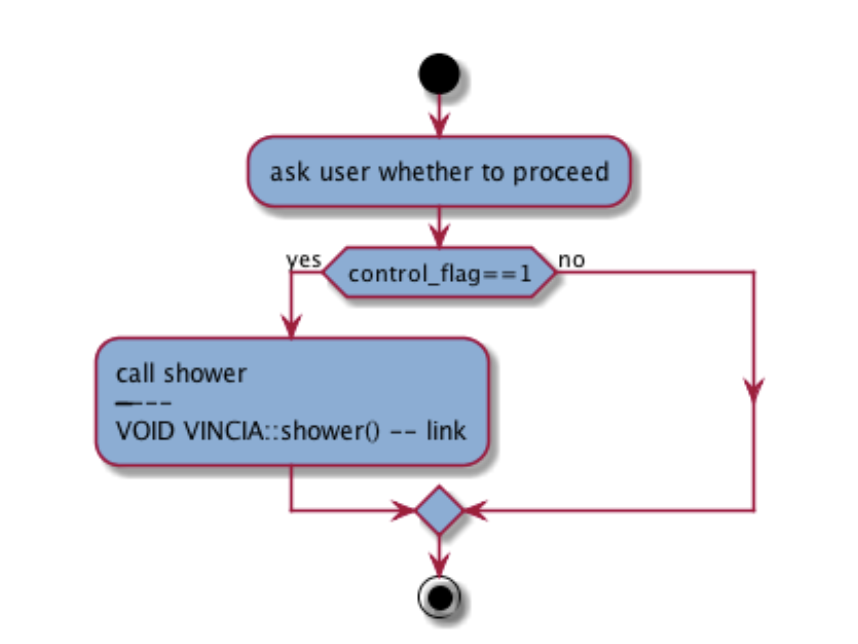
\includegraphics[scale=0.6]{assets/chapter3/Flowgen.png}
    \caption{\Cref{c++prog} converted to a flowchart with Flowgen. This example is not generated by us, but taken directly from~\cite{flowgen}.}
    \label{flowgenExample}
\end{figure}

\subsubsection{Online Tools}

\textbf{Code2Flow} is a tool that lets us create flowcharts with natural language, decorated with a C-inspired syntax. Their website states that we might get away with pasting syntactically correct C programs, but that this is purely incidental. This goes to show that the Code2Flow team have indeed developed a DSL with their own syntax. \\

Flowcharts created with Code2Flow have a few, consistent colours to differentiate parts of their corresponding programs. Start- and end expressions are displayed as red ovals, while all remaining expressions are displayed as blue rectangles. Conditionals, loops and match statements are displayed with red rhombuses, and comments are displayed with orange rectangles. \\

\begin{lstlisting}[caption={A Code2Flow program.}, captionpos=b, label={A Code2Flow program.}]
First statement;
Another statement;
if (conditional) {
  True statement;
} else {
  False statement; // Random comment
}
Last statement;
\end{lstlisting}

\Cref{A Code2Flow program.} shows a program written with Code2Flow, and \Cref{A Code2Flow flowchart.} presents the corresponding flowchart. As we can see, syntactically correct expressions are any combination of UTF-8 characters. Code2Flow will never warn us about syntactic errors, and will \textit{always} try to construct whatever flowchart it can. In turn, there is no clear way to test a Code2Flow program. \\

\begin{figure}[ht]
    \centering
    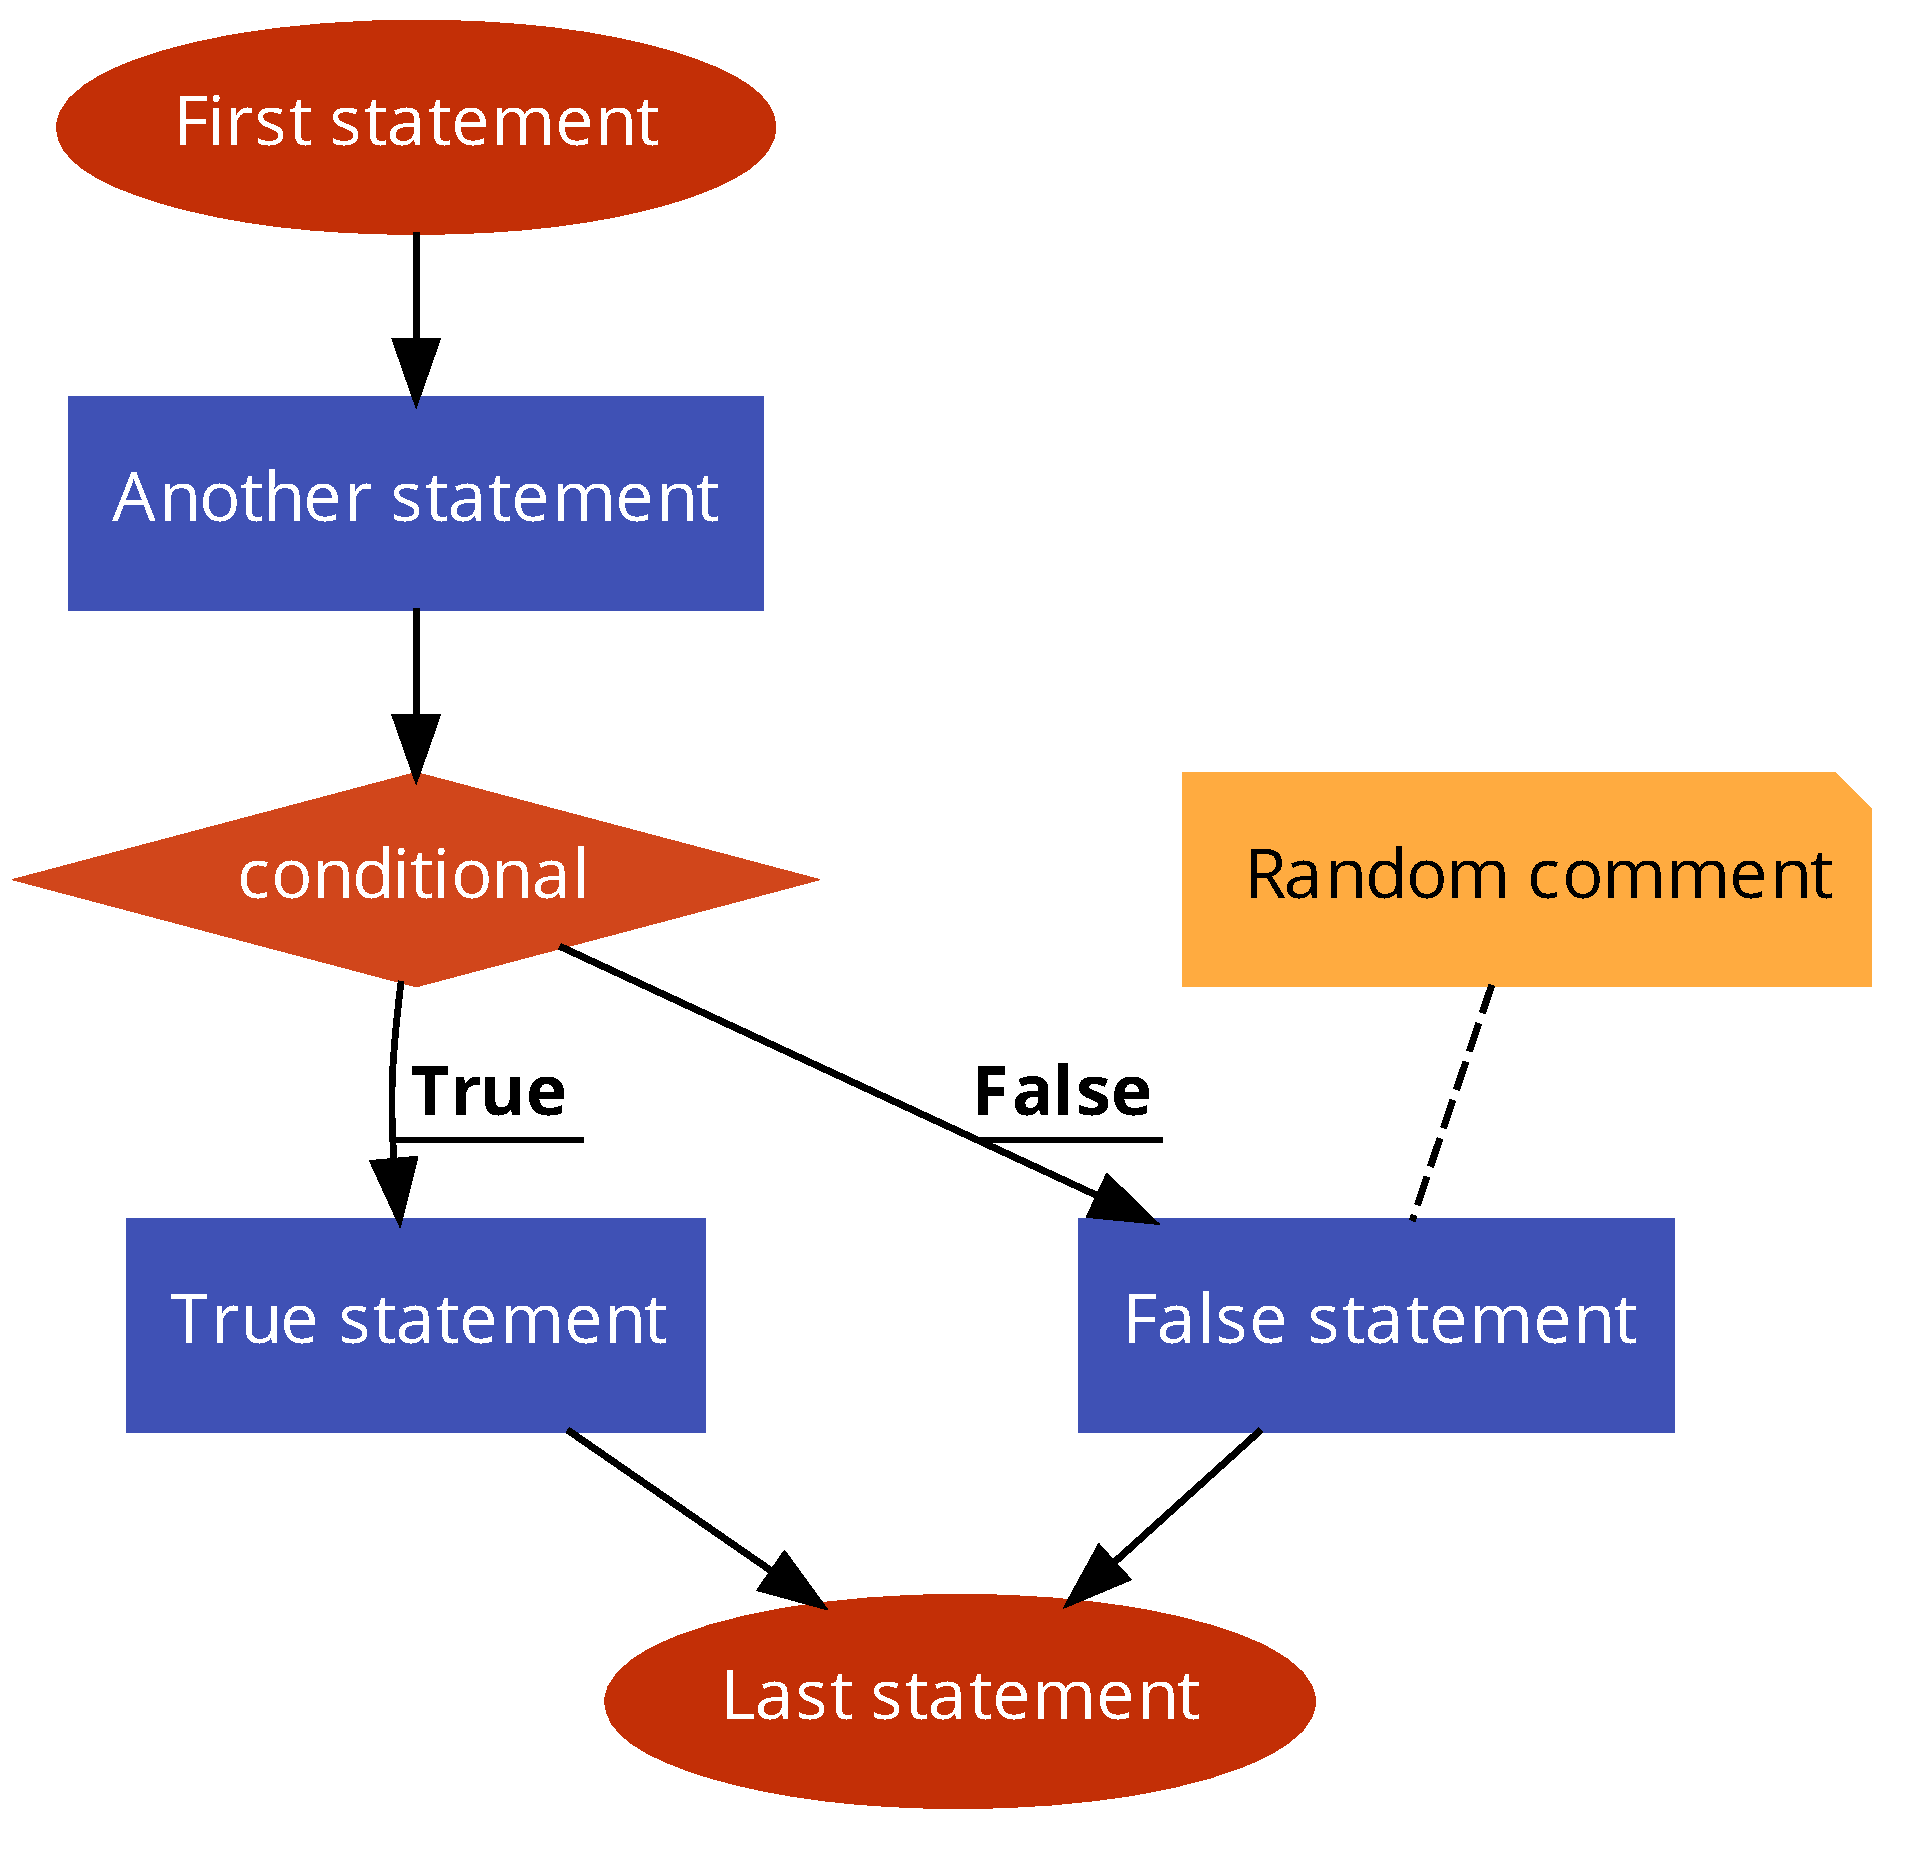
\includegraphics[scale=.28]{assets/chapter3/Code2FlowExample.pdf}
    \caption{The resulting flowchart from transpiling the Code2Flow code in \Cref{A Code2Flow program.}}
    \label{A Code2Flow flowchart.}
\end{figure}

If our C program inadvertently creates a ``correct'' flowchart, we can use a C compiler to test said program on the side. However, future changes to the C program are not guaranteed to successfully transpile to a new flowchart. \\

\textbf{Mermaid.js} is a DSL for rendering diagrams (including flowcharts) from a Markdown-inspired syntax. Even though we can construct many different diagrams with Mermaid.js, we will focus on the flowcharts. Like Code2Flow, they render flowcharts in real time. However, Mermaid.js \textit{will} warn us about syntax errors, and only re-render syntactically correct programs. \\

To construct a Mermaid.js flowchart, our source program must start with \texttt{flowchart TD}. Nodes can come in many different shapes, and are denoted by the types of brackets they use. For instance, \texttt{Node[ ]} displays a rectangle, \texttt{Node(( ))} displays a circle, and \texttt{Node\{ \}} displays a rhombus. Edges also come in many shapes: \texttt{$--$>} displays an arrow, \texttt{-.->} displays a dotted arrow, whilst \texttt{$---$} will display a simple link. \\

We can also add text to our nodes, by placing it within the brackets, like \texttt{Node[text]}. Arrows can also include text by breaking them up into two parts, like \texttt{$--$ text $--$>}.\footnote{The full documentation can be found here: \url{https://mermaid.js.org/syntax/flowchart.html}} \\

\begin{lstlisting}[caption={A mermaid.js program.}, captionpos=b, label={A mermaid.js program.}]
flowchart TD
    A([First statement])
        --> B[Another statement]
    B --> C{contidional}
    C -- True --> D[First statement]
    C -- False --> E[Second statement]
        %% Random comment
    D --> F([Last statement])
    E --> F
\end{lstlisting}

Just like with Code2Flow, the text inside these nodes can be anything. \Cref{A mermaid.js program.} shows a program written with Mermaid.js, and \Cref{A mermaid.js flowchart.} shows the corresponding flowchart. Contrary to Code2Flow, comments are ignored by the parser, and solely exist to aid the programmer. They must also be on their own lines. \\

The biggest drawback of Mermaid.js is that the syntax is very different from any programming language. This means pasting our source code will not yield any result, and we have to carefully translate our code every time. It also means that it is fully our responsability to maintain the abstraction level we want. Like Code2Flow, Mermaid.js has no way of letting us test our code. \\

\begin{figure}[ht]
    \centering
    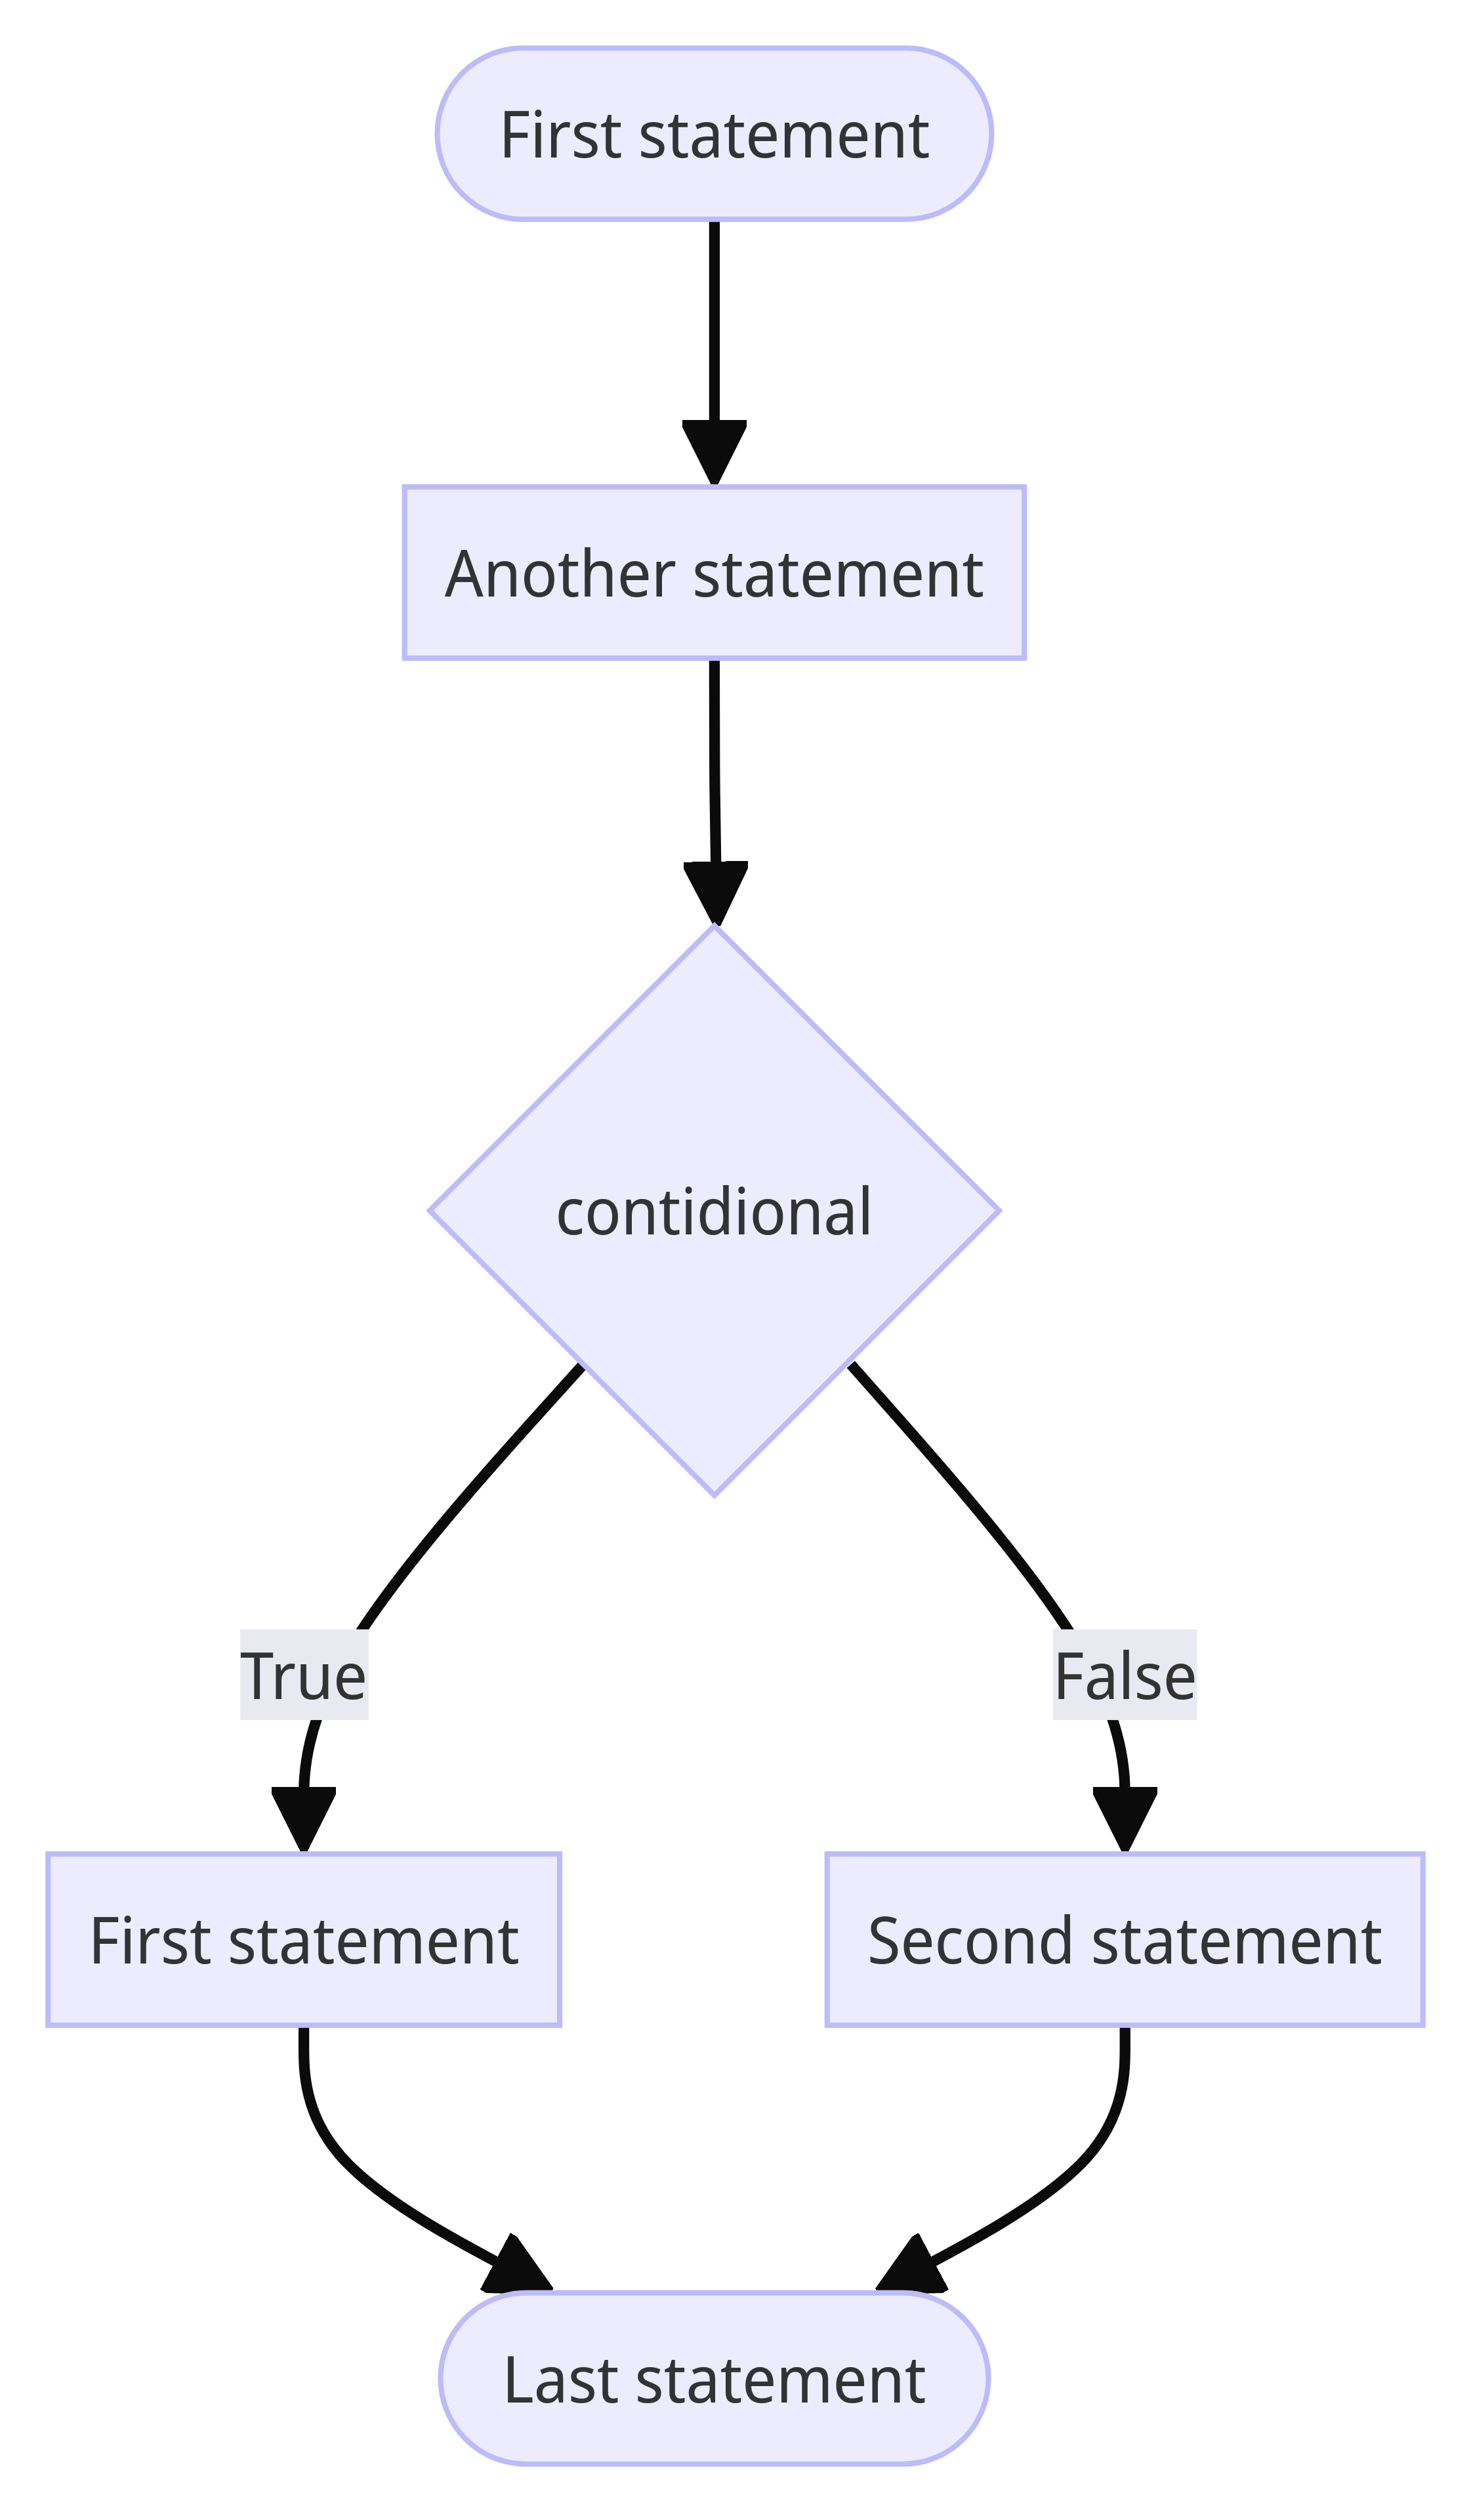
\includegraphics[scale=.07]{assets/chapter3/MermaidProgram.png}
    \caption{The resulting flowchart from transpiling the Mermaid.js code in \Cref{A mermaid.js program.}}
    \label{A mermaid.js flowchart.}
\end{figure}
